%%%%%%%%%%%%%%%%%%%%%%%%%%%%%%%%%%%%%%%%%%%%%%%%%%%%%%%%%%%%
%%  This Beamer template was created by Cameron Bracken.
%%  Anyone can freely use or modify it for any purpose
%%  without attribution.
%%
%%  Last Modified: January 9, 2009
%%

\documentclass[xcolor=x11names,compress]{beamer}

%% General document %%%%%%%%%%%%%%%%%%%%%%%%%%%%%%%%%%
\usepackage{graphicx}
\usepackage[utf8]{inputenc}
\usepackage[T1]{fontenc}
\usepackage[english]{babel}
\usepackage{amsmath,amssymb,amsthm,amsopn}
\usepackage{mathrsfs}
\usepackage{graphicx}
\usepackage{tikz}
\usepackage{array}
\usepackage{makecell}
%\usepackage[top=1cm,bottom=1cm]{geometry}
%\usepackage{listings}
%\usepackage{xcolor}
\usepackage{hyperref}
\hypersetup{
    colorlinks=true,
    linkcolor=blue,
    citecolor=red,
}

% Tikz style
\tikzset{round/.style={circle, draw=black, very thick, scale = 0.7}}
\tikzset{arrow/.style={->, >=latex}}
\tikzset{dashed-arrow/.style={->, >=latex, dashed}}

\newtheoremstyle{break}%
{}{}%
{\itshape}{}%
{\bfseries}{}%  % Note that final punctuation is omitted.
{\newline}{}

\newtheoremstyle{sc}%
{}{}%
{}{}%
{\scshape}{}%  % Note that final punctuation is omitted.
{\newline}{}

\theoremstyle{break}
\newtheorem{thm}{Theorem}[section]
\newtheorem{lm}[thm]{Lemma}
\newtheorem{prop}[thm]{Proposition}
\newtheorem{cor}[thm]{Corollary}

\theoremstyle{sc}
\newtheorem{exo}{Exercice}

\theoremstyle{definition}
\newtheorem{defi}[thm]{Definition}
\newtheorem{ex}[thm]{Example}

\theoremstyle{remark}
\newtheorem{rem}[thm]{Remark}

% Raccourcis pour les opérateurs mathématiques (les espaces avant-après sont
% modifiés pour mieux rentrer dans les codes mathématiques usuels)
\DeclareMathOperator{\Ker}{Ker}
\DeclareMathOperator{\Id}{Id}
\DeclareMathOperator{\Img}{Im}
\DeclareMathOperator{\Card}{Card}
\DeclareMathOperator{\Vect}{Vect}
\DeclareMathOperator{\Tr}{Tr}
\DeclareMathOperator{\Mod}{mod}
\DeclareMathOperator{\Ord}{Ord}
\DeclareMathOperator{\ppcm}{ppcm}
\DeclareMathOperator{\Minpoly}{Minpoly}
\DeclareMathOperator{\Gal}{Gal}


% Nouvelles commandes
\newcommand{\ps}[2]{\left\langle#1,#2\right\rangle}
\newcommand{\ent}[2]{[\![#1,#2]\!]}
\newcommand{\diff}{\mathop{}\!\mathrm{d}}
\newcommand{\ie}{\emph{i.e. }}
\newcommand{\eg}{\emph{e.g. }}
\newcommand{\embed}[2]{\phi_{#1\hookrightarrow#2}}
%%%%%%%%%%%%%%%%%%%%%%%%%%%%%%%%%%%%%%%%%%%%%%%%%%%%%%


%% Beamer Layout %%%%%%%%%%%%%%%%%%%%%%%%%%%%%%%%%%
\useoutertheme[subsection=false,shadow]{miniframes}
\useinnertheme{default}
\usefonttheme{serif}
\usepackage{palatino}
\setbeamertemplate{navigation symbols}{}%remove navigation symbols
\setbeamertemplate{footline}[frame number]


\setbeamerfont{title like}{shape=\scshape}
\setbeamerfont{frametitle}{shape=\scshape}

\setbeamercolor*{lower separation line head}{bg=DeepSkyBlue4} 
% \setbeamercolor*{normal text}{fg=black,bg=white} 
% \setbeamercolor*{alerted text}{fg=red} 
% \setbeamercolor*{example text}{fg=black} 
% \setbeamercolor*{structure}{fg=black} 
%  
\setbeamercolor*{palette tertiary}{fg=black,bg=black!10} 
\setbeamercolor*{palette quaternary}{fg=black,bg=black!10} 
% 
% \renewcommand{\(}{\begin{columns}}
% \renewcommand{\)}{\end{columns}}
% \newcommand{\<}[1]{\begin{column}{#1}}
% \renewcommand{\>}{\end{column}}

\AtBeginSection[]{
  \begin{frame}
  \vfill
  \centering
  \begin{beamercolorbox}[sep=8pt,center,shadow=false,rounded=true]{title}
    \usebeamerfont{title}\secname\par%
  \end{beamercolorbox}
  \vfill
  \end{frame}
}

%%%%%%%%%%%%%%%%%%%%%%%%%%%%%%%%%%%%%%%%%%%%%%%%%%




\begin{document}


%%%%%%%%%%%%%%%%%%%%%%%%%%%%%%%%%%%%%%%%%%%%%%%%%%%%%%
%%%%%%%%%%%%%%%%%%%%%%%%%%%%%%%%%%%%%%%%%%%%%%%%%%%%%%
\begin{frame}
  \title{Lattices of compatibly embedded finite fields}
%\subtitle{SUBTITLE}
  \author{Edouard Rousseau}
\date{GT BAC\\\today}
\titlepage
\end{frame}

%%%%%%%%%%%%%%%%%%%%%%%%%%%%%%%%%%%%%%%%%%%%%%%%%%%%%%
%%%%%%%%%%%%%%%%%%%%%%%%%%%%%%%%%%%%%%%%%%%%%%%%%%%%%%
\begin{frame}{Contents}
  \tableofcontents%[hideallsubsections]
\end{frame}

%%%%%%%%%%%%%%%%%%%%%%%%%%%%%%%%%%%%%%%%%%%%%%%%%%%%%%
%%%%%%%%%%%%%%%%%%%%%%%%%%%%%%%%%%%%%%%%%%%%%%%%%%%%%%
\section{The embedding problem}
\subsection{The problem}
\begin{frame}{The embedding problem}
  \begin{itemize}
    \item $f$ irreducible polynomial of degree $m$ in
      $\mathbb{F}_p[X]$
    \item $g$ irreducible polynomial of degree $n$ in $\mathbb{F}_p[Y]$
    \item $m\,|\,n$
    \item $E = \mathbb{F}_p[X]/(f(X))$
    \item $F = \mathbb{F}_p[Y]/(g(Y))$
  \end{itemize}
  \[
    E \cong \mathbb{F}_{p^m} \hookrightarrow \mathbb{F}_{p^n}\cong F
  \]
  \begin{itemize}
    \item \textcolor{purple}{\textbf{Embedding problem:}} how to compute the
      embedding from $E$ to $F$ ?
  \end{itemize}
\end{frame}
\begin{frame}{Description and evaluation}
  \textcolor{purple}{\textbf{Two steps:}}
  \begin{itemize}
    \item Description: find $\alpha_1, \alpha_2$ such that
      \begin{itemize}
        \item $E = \mathbb{F}_p(\alpha_1)$
        \item \emph{there exists} an embedding $\phi:E\to F$ mapping
          $\alpha_1\mapsto\alpha_2$
      \end{itemize}
    \item Evaluation
      \begin{itemize}
        \item Compute $\phi(\gamma)\in F$ for $\gamma\in E$
        \item Test if $\delta\in\phi(E)$ for $\delta\in F$
        \item If $\delta\in\phi(E)$, compute $\phi^{-1}(\delta)\in E$
      \end{itemize}
  \end{itemize}
\end{frame}
\subsection{Description}
\begin{frame}{Description - Naive algorithm}
  \textcolor{purple}{\textbf{Context:}}
  \[
    E = \mathbb{F}_p[X]/(f)\phantom{and}F=\mathbb{F}_p[Y]/(g)
  \]
  
  \textcolor{purple}{\textbf{Algorithm:}}
  \begin{itemize}
    \item Find a root $\rho$ of $f$ in $F$
    \item $\alpha_1 = \overline X$
    \item $\alpha_2 = \rho$
  \end{itemize}
  % Complexity strictly larger than \textcolor{violet}{\textbf{$\widetilde
  % O(n^2)$}}
\end{frame}
\begin{frame}{Description - Allombert's algorithm ($m\,|\,p-1$)}
Assume $m\,|\,p-1$.
  \begin{itemize}
    \item $\exists \zeta\in\mathbb{F}_p$, primitive $m$-th root of unity
    \item Find such a $\zeta$
    \item Solve $\sigma(x) = \zeta x$ in $E$, where $\sigma:=$
      Frobenius automorphism (Hilbert 90)
      \begin{itemize}
        \item Denote by $\alpha_1$ a solution
      \end{itemize}
    \item Solve $\sigma(y) = \zeta y$ in $F$
      \begin{itemize}
        \item Denote by $\alpha_2$ a solution
      \end{itemize}
  \end{itemize}
  \textcolor{purple}{\textbf{Facts:}}
  \begin{itemize}
    \item $E=\mathbb{F}_p(\alpha_1)$%, $F=\mathbb{F}_p(\alpha_2)$
  \item $a_1:=\alpha_1^m\in\mathbb{F}_p$, $a_2:=\alpha_2^m\in\mathbb{F}_p$
    \item $a_1/a_2$ is a $m$-th power in $\mathbb{F}_p$
      \begin{itemize}
        \item Compute $c\in\mathbb{F}_p$ such that $c^m=a_1/a_2$
      \end{itemize}
  \end{itemize}
  Take the map $\alpha_1\mapsto c\alpha_2$
\end{frame}
\begin{frame}{Description - Allombert's algorithm}
  In general:
  \begin{itemize}
    \item We do not necessarily have primitive $m$-th roots of unity $\zeta$ in $\mathbb{F}_p$
    \item We work in $E\otimes_{\mathbb{F}_p}C$ and
      $F\otimes_{\mathbb{F}_p}C$, where $C$ is a finite extension of
      $\mathbb{F}_p$ containing primitive $m$-th roots of unity
    \item We use the same kind of results to find $\alpha_1$, $\alpha_2$
  \end{itemize}
  
\end{frame}

\section{The compatibility problem}
\subsection{The problem}
\begin{frame}{The compatibility problem}
  \textcolor{purple}{\textbf{Context:}}
  \begin{itemize}
    \item $E$, $F$, $G$ fields
    \item $E$ subfield of $F$ and $F$ subfield of $G$
    \item $\phi_{E\hookrightarrow F}$, $\embed{F}{G}$,
      $\embed{E}{G}$ embeddings
  \end{itemize}
  \begin{figure}
    \centering
    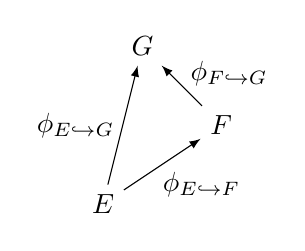
\begin{tikzpicture}
      \node (E) at (0, 0) {$E$}; 
      \node (F) at (1.5, 1) {$F$}; 
      \node (G) at (0.5, 2) {$G$}; 

      \draw[arrow] (E) -- (F);
      \draw[arrow] (E) -- (G);
      \draw[arrow] (F) -- (G);

      \node (f12) at (1.25, 0.25) {$\embed{E}{F}$};
      \node (f13) at (-0.35, 1) {$\embed{E}{G}$};
      \node (f23) at (1.6, 1.65) {$\embed{F}{G}$};
    \end{tikzpicture}
  \end{figure}
  \[
    \textcolor{purple}{\embed{F}{G}\circ\embed{E}{F}\overset{?}{=}\embed{E}{G}}
  \]
\end{frame}
\begin{frame}{The compatibility problem II}
   \begin{figure}
    \centering
    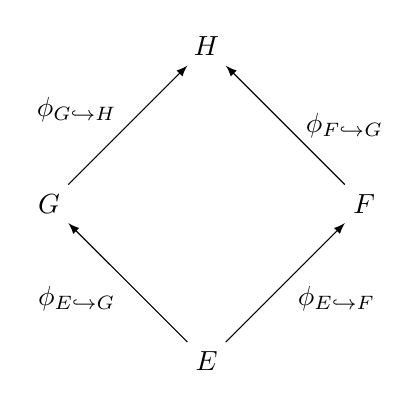
\begin{tikzpicture}
      \node (E) at (0, 0) {$E$}; 
      \node (F) at (2, 2) {$F$}; 
      \node (G) at (-2, 2) {$G$}; 
      \node (H) at (0, 4) {$H$}; 

      \draw[arrow] (E) -- (F);
      \draw[arrow] (E) -- (G);
      \draw[arrow] (G) -- (H);
      \draw[arrow] (F) -- (H);

      \node (f12) at (1.65, 0.8) {$\embed{E}{F}$};
      \node (f13) at (-1.65, 0.8) {$\embed{E}{G}$};
      \node (f24) at (1.75, 3) {$\embed{F}{G}$};
      \node (f34) at (-1.65, 3.2) {$\embed{G}{H}$};
    \end{tikzpicture}
  \end{figure}
  \[
    \textcolor{purple}{\embed{G}{H}\circ\embed{E}{G}\overset{?}{=}\embed{F}{H}\circ\embed{E}{F}}
  \]
\end{frame}

\subsection{Bosma, Cannon and Steel framework}
\begin{frame}{Bosma, Cannon and Steel}
  \begin{itemize}
    \item Allows to work with arbitrary, user-defined finite fields
    \item Allows to build the embeddings in arbitrary order
    \item Used in MAGMA
  \end{itemize}
\end{frame}
\begin{frame}{Bosma, Cannon and Steel framework (theory)}
  \textcolor{purple}{\textbf{First example}} 
  \begin{figure}
    \centering
    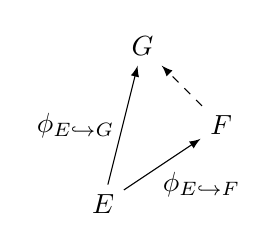
\begin{tikzpicture}
      \node (E) at (0, 0) {$E$}; 
      \node (F) at (1.5, 1) {$F$}; 
      \node (G) at (0.5, 2) {$G$}; 

      \draw[arrow] (E) -- (F);
      \draw[arrow] (E) -- (G);
      \draw[dashed-arrow] (F) -- (G);

      \node (f12) at (1.25, 0.25) {$\embed{E}{F}$};
      \node (f13) at (-0.35, 1) {$\embed{E}{G}$};
    \end{tikzpicture}
  \end{figure}
  \begin{itemize}
    \item Take $\embed{F}{G}'$ an arbitrary embedding between $F$ and
      $G$
    \item Find $\sigma\in\Gal(G/\mathbb{F}_p)$ such that
      $\sigma\circ\embed{F}{G}'\circ\embed{E}{F}=\embed{E}{G}$
    \item Set $\embed{F}{G}:=\sigma\circ\embed{F}{G}'$
    \item There are $|\Gal(F/E)|$ compatible morphisms
  \end{itemize}
\end{frame}
\begin{frame}{Bosma, Cannon and Steel framework (theory)}
  What about several subfields $E_1, E_2, \dots, E_r$ ?
  \begin{itemize}
    \item We impose some conditions on the lattice 
      \begin{itemize}
        \item[CE1] (Unicity) At most one morphism $\embed{E}{F}$
        \item[CE2] (Reflexivity) For each $E$, $\embed{E}{E}=\Id_E$
        \item[CE3] (Invertibility) For each pair $(E, F)$ with $E\cong F$,
          $\embed{E}{F}=\embed{F}{E}^{-1}$ 
        \item[CE4] (Transitivity) For any triple $(E, F, G)$ with $E$
          subfield of $F$ and $F$ subfield of $G$, if we have
         computed $\embed{E}{F}$ and $\embed{F}{G}$, then
         $\embed{E}{G}=\embed{F}{G}\circ\embed{E}{F}$
       \item[CE5] (Intersections) For any triple $(E, F, G)$ with $E$ and $F$
         subfields of $G$, we have that the field $S=E\cap F$ is embedded in
         $E$ and $F$, \ie we have computed $\embed{S}{E}$ and
         $\embed{S}{F}$
      \end{itemize}
  \end{itemize}
\end{frame}
\begin{frame}{Bosma, Cannon and Steel framework (theory)}
    \begin{figure}
    \centering
    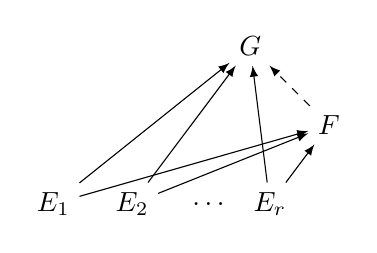
\begin{tikzpicture}
      \node (E1) at (-2, 0) {$E_1$}; 
      \node (E2) at (-1, 0) {$E_2$}; 
      \node (Er) at (0.75, 0) {$E_r$}; 
      \node (F) at (1.5, 1) {$F$}; 
      \node (G) at (0.5, 2) {$G$}; 
      \node (p) at (0, 0) {$\dots$};

      \draw[arrow] (E1) -- (F);
      \draw[arrow] (E1) -- (G);
      \draw[arrow] (E2) -- (F);
      \draw[arrow] (E2) -- (G);
      \draw[arrow] (Er) -- (F);
      \draw[arrow] (Er) -- (G);
      \draw[dashed-arrow] (F) -- (G);
    \end{tikzpicture}
  \end{figure}
  \begin{itemize}
    \item Set $F'$ the field generated by the fields $E_i$ in $F$
    \item Set $G'$ the field generated by the fields $E_i$ in $G$
  \end{itemize}
  \begin{thm}
There exists a unique isomorphism $\chi:F'\to G'$ that is compatible with all
embeddings, \ie such that for all $i$,
$\embed{E_i}{G'}=\chi\circ\embed{E_i}{F'}$.
  \end{thm}
\end{frame}
\begin{frame}{Bosma, Cannon and Steel framework (theory)}
   \begin{figure}
    \centering
     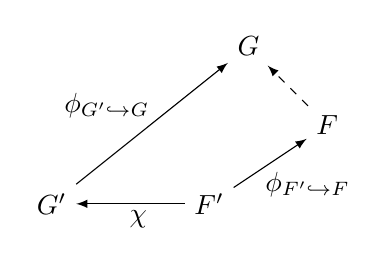
\begin{tikzpicture}
      \node (Fp) at (0, 0) {$F'$}; 
      \node (F) at (1.5, 1) {$F$}; 
      \node (Gp) at (-2, 0) {$G'$}; 
      \node (G) at (0.5, 2) {$G$}; 

      \draw[arrow] (Fp) -- (F);
      \draw[arrow] (Gp) -- (G);
      \draw[arrow] (Fp) -- (Gp);
      \draw[dashed-arrow] (F) -- (G);

      \node (chi) at (-0.9, -0.2) {$\chi$};
      \node (f12) at (1.25, 0.25) {$\embed{F'}{F}$};
      \node (GGp) at (-1.3, 1.25) {$\embed{G'}{G}$};

    \end{tikzpicture}
    \phantom{and now}
   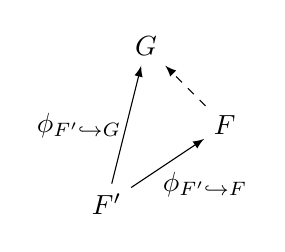
\begin{tikzpicture}
      \node (E) at (0, 0) {$F'$}; 
      \node (F) at (1.5, 1) {$F$}; 
      \node (G) at (0.5, 2) {$G$}; 

      \draw[arrow] (E) -- (F);
      \draw[arrow] (E) -- (G);
      \draw[dashed-arrow] (F) -- (G);

      \node (f12) at (1.25, 0.25) {$\embed{F'}{F}$};
      \node (f13) at (-0.35, 1) {$\embed{F'}{G}$};
    \end{tikzpicture}
  \end{figure}
  \begin{itemize}
    \item We have $|\Gal(F/F')|$ compatible morphisms
  \end{itemize}
\end{frame}
\begin{frame}{Bosma, Cannon and Steel framework (practice)}
  \begin{itemize}
    \item Use the naive embedding algorithm 
  \end{itemize}
   \begin{figure}
    \centering
    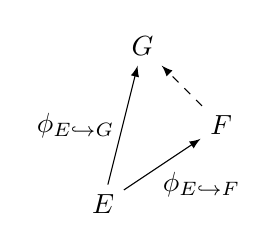
\begin{tikzpicture}
      \node (E) at (0, 0) {$E$}; 
      \node (F) at (1.5, 1) {$F$}; 
      \node (G) at (0.5, 2) {$G$}; 

      \draw[arrow] (E) -- (F);
      \draw[arrow] (E) -- (G);
      \draw[dashed-arrow] (F) -- (G);

      \node (f12) at (1.25, 0.25) {$\embed{E}{F}$};
      \node (f13) at (-0.35, 1) {$\embed{E}{G}$};
    \end{tikzpicture}
  \end{figure}

  \begin{itemize}
    \item Consider $\alpha$ such that $F=\mathbb{F}_p(\alpha)$
    \item Take $\rho$ a root of $\embed{E}{G}(\Minpoly_E(\alpha))$
    \item Map $\alpha\mapsto\rho$ and
      \[
        \embed{F}{G}(\sum_{i=0}^{[F:E]-1}e_i\alpha^i) =
        \sum_{i=0}^{[F:E]-1}\embed{E}{G}(e_i)\rho^i
      \]
  \end{itemize}
\end{frame}
\begin{frame}{Bosma, Cannon and Steel framework (practice)}
     \begin{figure}
    \centering
    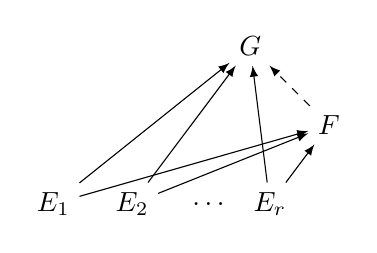
\begin{tikzpicture}
      \node (E1) at (-2, 0) {$E_1$}; 
      \node (E2) at (-1, 0) {$E_2$}; 
      \node (Er) at (0.75, 0) {$E_r$}; 
      \node (F) at (1.5, 1) {$F$}; 
      \node (G) at (0.5, 2) {$G$}; 
      \node (p) at (0, 0) {$\dots$};

      \draw[arrow] (E1) -- (F);
      \draw[arrow] (E1) -- (G);
      \draw[arrow] (E2) -- (F);
      \draw[arrow] (E2) -- (G);
      \draw[arrow] (Er) -- (F);
      \draw[arrow] (Er) -- (G);
      \draw[dashed-arrow] (F) -- (G);
    \end{tikzpicture}
  \end{figure}
   \begin{itemize}
    \item Consider $\alpha$ such that $F=\mathbb{F}_p(\alpha)$
    \item Take $\rho$ a root of
      $\gcd_i(\embed{E_i}{G}(\Minpoly_{E_i}(\alpha)))$
    \item Map $\alpha\mapsto\rho$
  \end{itemize}
\end{frame}
\begin{frame}{Bosma, Cannon and Steel framework}
  To embed $F$ in $G$:
  \begin{enumerate}
    \item For each subfield $S$ of $G$, if $S\cap F$ is not embedded in $S$ and
      $F$, if not, embed it
    \item embed $F$ in $G$ using the method seen before
    \item take the transitive closure
  \end{enumerate}
\end{frame}
\begin{frame}{Bosma, Cannon and Steel framework}
  Some configurations with triangles:
  \begin{figure}
    \centering
    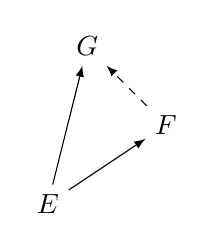
\begin{tikzpicture}
      \node (E) at (0, 0) {$E$}; 
      \node (F) at (1.5, 1) {$F$}; 
      \node (G) at (0.5, 2) {$G$}; 

      \draw[arrow] (E) -- (F);
      \draw[arrow] (E) -- (G);
      \draw[dashed-arrow] (F) -- (G);
    \end{tikzpicture}
    \phantom{and}
    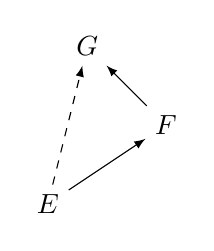
\begin{tikzpicture}
      \node (E) at (0, 0) {$E$}; 
      \node (F) at (1.5, 1) {$F$}; 
      \node (G) at (0.5, 2) {$G$}; 

      \draw[arrow] (E) -- (F);
      \draw[dashed-arrow] (E) -- (G);
      \draw[arrow] (F) -- (G);

    \end{tikzpicture}
    \phantom{and}
    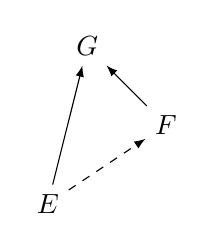
\begin{tikzpicture}
      \node (E) at (0, 0) {$E$}; 
      \node (F) at (1.5, 1) {$F$}; 
      \node (G) at (0.5, 2) {$G$}; 

      \draw[dashed-arrow] (E) -- (F);
      \draw[arrow] (E) -- (G);
      \draw[arrow] (F) -- (G);

    \end{tikzpicture}
  \end{figure}
  \uncover<2->{
  \begin{figure}
    \centering
    \begin{tikzpicture}
      \node (E) at (0, 0) {$E$}; 
      \node (F) at (1.5, 1) {$F$}; 
      \node (G) at (0.5, 2) {$G$}; 

      \draw[arrow] (E) -- (G);
      \draw[dashed-arrow] (F) -- (G);
    \end{tikzpicture}
    \phantom{and}
    \begin{tikzpicture}
      \node (E) at (0, 0) {$E$}; 
      \node (F) at (1.5, 1) {$F$}; 
      \node (G) at (0.5, 2) {$G$}; 

      \draw[dashed-arrow] (E) -- (G);
      \draw[arrow] (F) -- (G);
    \end{tikzpicture}
  \end{figure}
}

\end{frame}
\begin{frame}{Bosma, Cannon and Steel framework}
  An example of what can happen with the intersections:

  \begin{figure}
    \centering
    \begin{tikzpicture}[scale=.8]
      
      \node (60) at (0, 0) {$\mathbb{F}_{p^{60}}$};
      \node (120) at (2, 2) {$\mathbb{F}_{p^{120}}$};
      \node (60) at (0, 0) {$\mathbb{F}_{p^{60}}$};
      \node (30) at (-2, -2) {$\mathbb{F}_{p^{30}}$};
      \node (40) at (4, 0) {$\mathbb{F}_{p^{40}}$};
      \node (6) at (-4, -4) {$\mathbb{F}_{p^{6}}$};

      \draw[arrow] (6) -- (30);
      \draw[arrow] (30) -- (60);
      \draw[arrow] (40) -- (120);
      \draw[dashed-arrow] (60) -- (120);

      \uncover<2->{
        \node (20) at (2, -2) {$\mathbb{F}_{p^{20}}$};
        \draw[arrow] (20) -- (40);
        \draw[dashed-arrow] (20) -- (60);
      }

      \uncover<3->{
        \node (10) at (0, -4) {$\mathbb{F}_{p^{10}}$};
        \draw[arrow] (10) -- (20);
        \draw[dashed-arrow] (10) -- (30);
      }

      \uncover<4->{
        \node (2) at (-2, -6) {$\mathbb{F}_{p^{2}}$};
        \draw[arrow] (2) -- (10);
        \draw[arrow] (2) -- (6);
      }

      \uncover<5->{
        \draw[arrow] (10) -- (30);
      }
      \uncover<6->{
        \draw[arrow] (20) -- (60);
      }
      \uncover<7->{
        \draw[arrow] (60) -- (120);
      }
    \end{tikzpicture}
  \end{figure}
  
\end{frame}
\subsection{Computing an isomorphism with a common subfield}
\begin{frame}{Computing an isomorphism with a common subfield}
  \begin{itemize}
    \item We want to embed $E$ in $F$
      \begin{itemize}
        \item additionnal information: $S$ is a field embedded in $E$ and $F$
      \end{itemize}
   \item We factor a degree $[E:S]$ polynomial in $F$, instead of a degree
     $[E:\mathbb{F}_p]$ polynomial in $F$.
   \item Several common subfields $S_1, S_2, \dots, S_r$ are equivalent to the
     field $S'$ generated by the $S_i$ in $E$
  \end{itemize}
\end{frame}
\begin{frame}{Some questions}
  \begin{itemize}
    \item Can we use Bosma, Cannon and Steel framework with a more efficient
      algorithm ? (\eg Allombert's)
    \item Can we use a similar common subfield trick with Allombert's
      algorithm ?
  \end{itemize}
\end{frame}
\begin{frame}
  \begin{center}
    \huge{Thank you for your attention !}
  \end{center}
\end{frame}
\end{document}
